\chapter{Dataset preprocessing and features extraction}\label{chap4}

In the previous chapter we introduced the concepts of Artificial Neural Networks in the Machine learning framework for the classification task. In this chapter we will discuss how, starting from the "raw" dataset we can extract, clean and preprocess the main features which will compose the final dataset for the training of our classifier model.

The datasets introduced in \chapref{chap3} can not be in fact directly used for the training. These datasets are in fact save as \texttt{pcap} files, a format used to save the information about the traffic of a network, which can not be directly interfaced with a ANN which requires as input a set of numeric values. In this chapter we will also describe which are the main features we are interested in studying in order to solve the identification task and list the devices considered to create the final dataset.

\section{Traffic stream time series creation}

Since all the traffic information is contained in \texttt{pcap} files it is necessary to extract and convert this information to a numeric format in order to utilize it as input of the model.
To do this we use the WireShark suite which allows to inspect \textit{pcap} files and offers various tools to process them. In particular the \texttt{tshark} command line tools allows to extract a time series of the traffic stream.

Using this tool the traffic time series are extracted in the following way: for each device listed in \tabref{tab:4sicsdevlist} and \tabref{tab:iotdevlist} we use its IP or MAC address to respectively filter the traffic data. After this for each device we export to a simple text file the total time series. To avoid notation issues in the following we will refer to the total time series of a device as ${\tilde{X}_i^j}$, where $i$ is a time index representing the value of the timeseries at a specif time and $j$ is an index representing the particular feature considered. 
Each device is then represented by a multivariate timeseries. The features considered for this work, alongisde with the associated j-index, are reported in the following:
\begin{itemize}[noitemsep]
    \item ${\tilde{X}_i^1}$: Number of packages transferred \textbf{from} the specific device to the whole network
    \item ${\tilde{X}_i^2}$: Number of packages transferred \textbf{to} the specific device from the whole network
    \item ${\tilde{X}_i^3}$: Bytes transferred \textbf{from} the specific device to the whole network
    \item ${\tilde{X}_i^4}$: Bytes transferred \textbf{to} the specific device from the whole network
\end{itemize}

The choice of requesting a separate time series of the traffic from/to a specific device is particularly important since it allows the classifier to distinguish the behaviour of devices with mostly output traffic (e.g. sensors) from devices with mostly input traffic (e.g. control devices).
In \figref{fig:ts_example_4sics} and \figref{fig:ts_example_iot} an example of the time series extracted from some devices of the 4SICS and IoT dataset are respectively shown. It is important to notice that the IoT device time series is very short if compared to the 4SICS one; this fact is not purely coincidential, in fact all the time series from the IoT dataset present a small number of elements due to the small amount of captured traffic in the relative \texttt{pcap} file.


\begin{figure}[!h]
\vspace{-5mm}
    \centering
   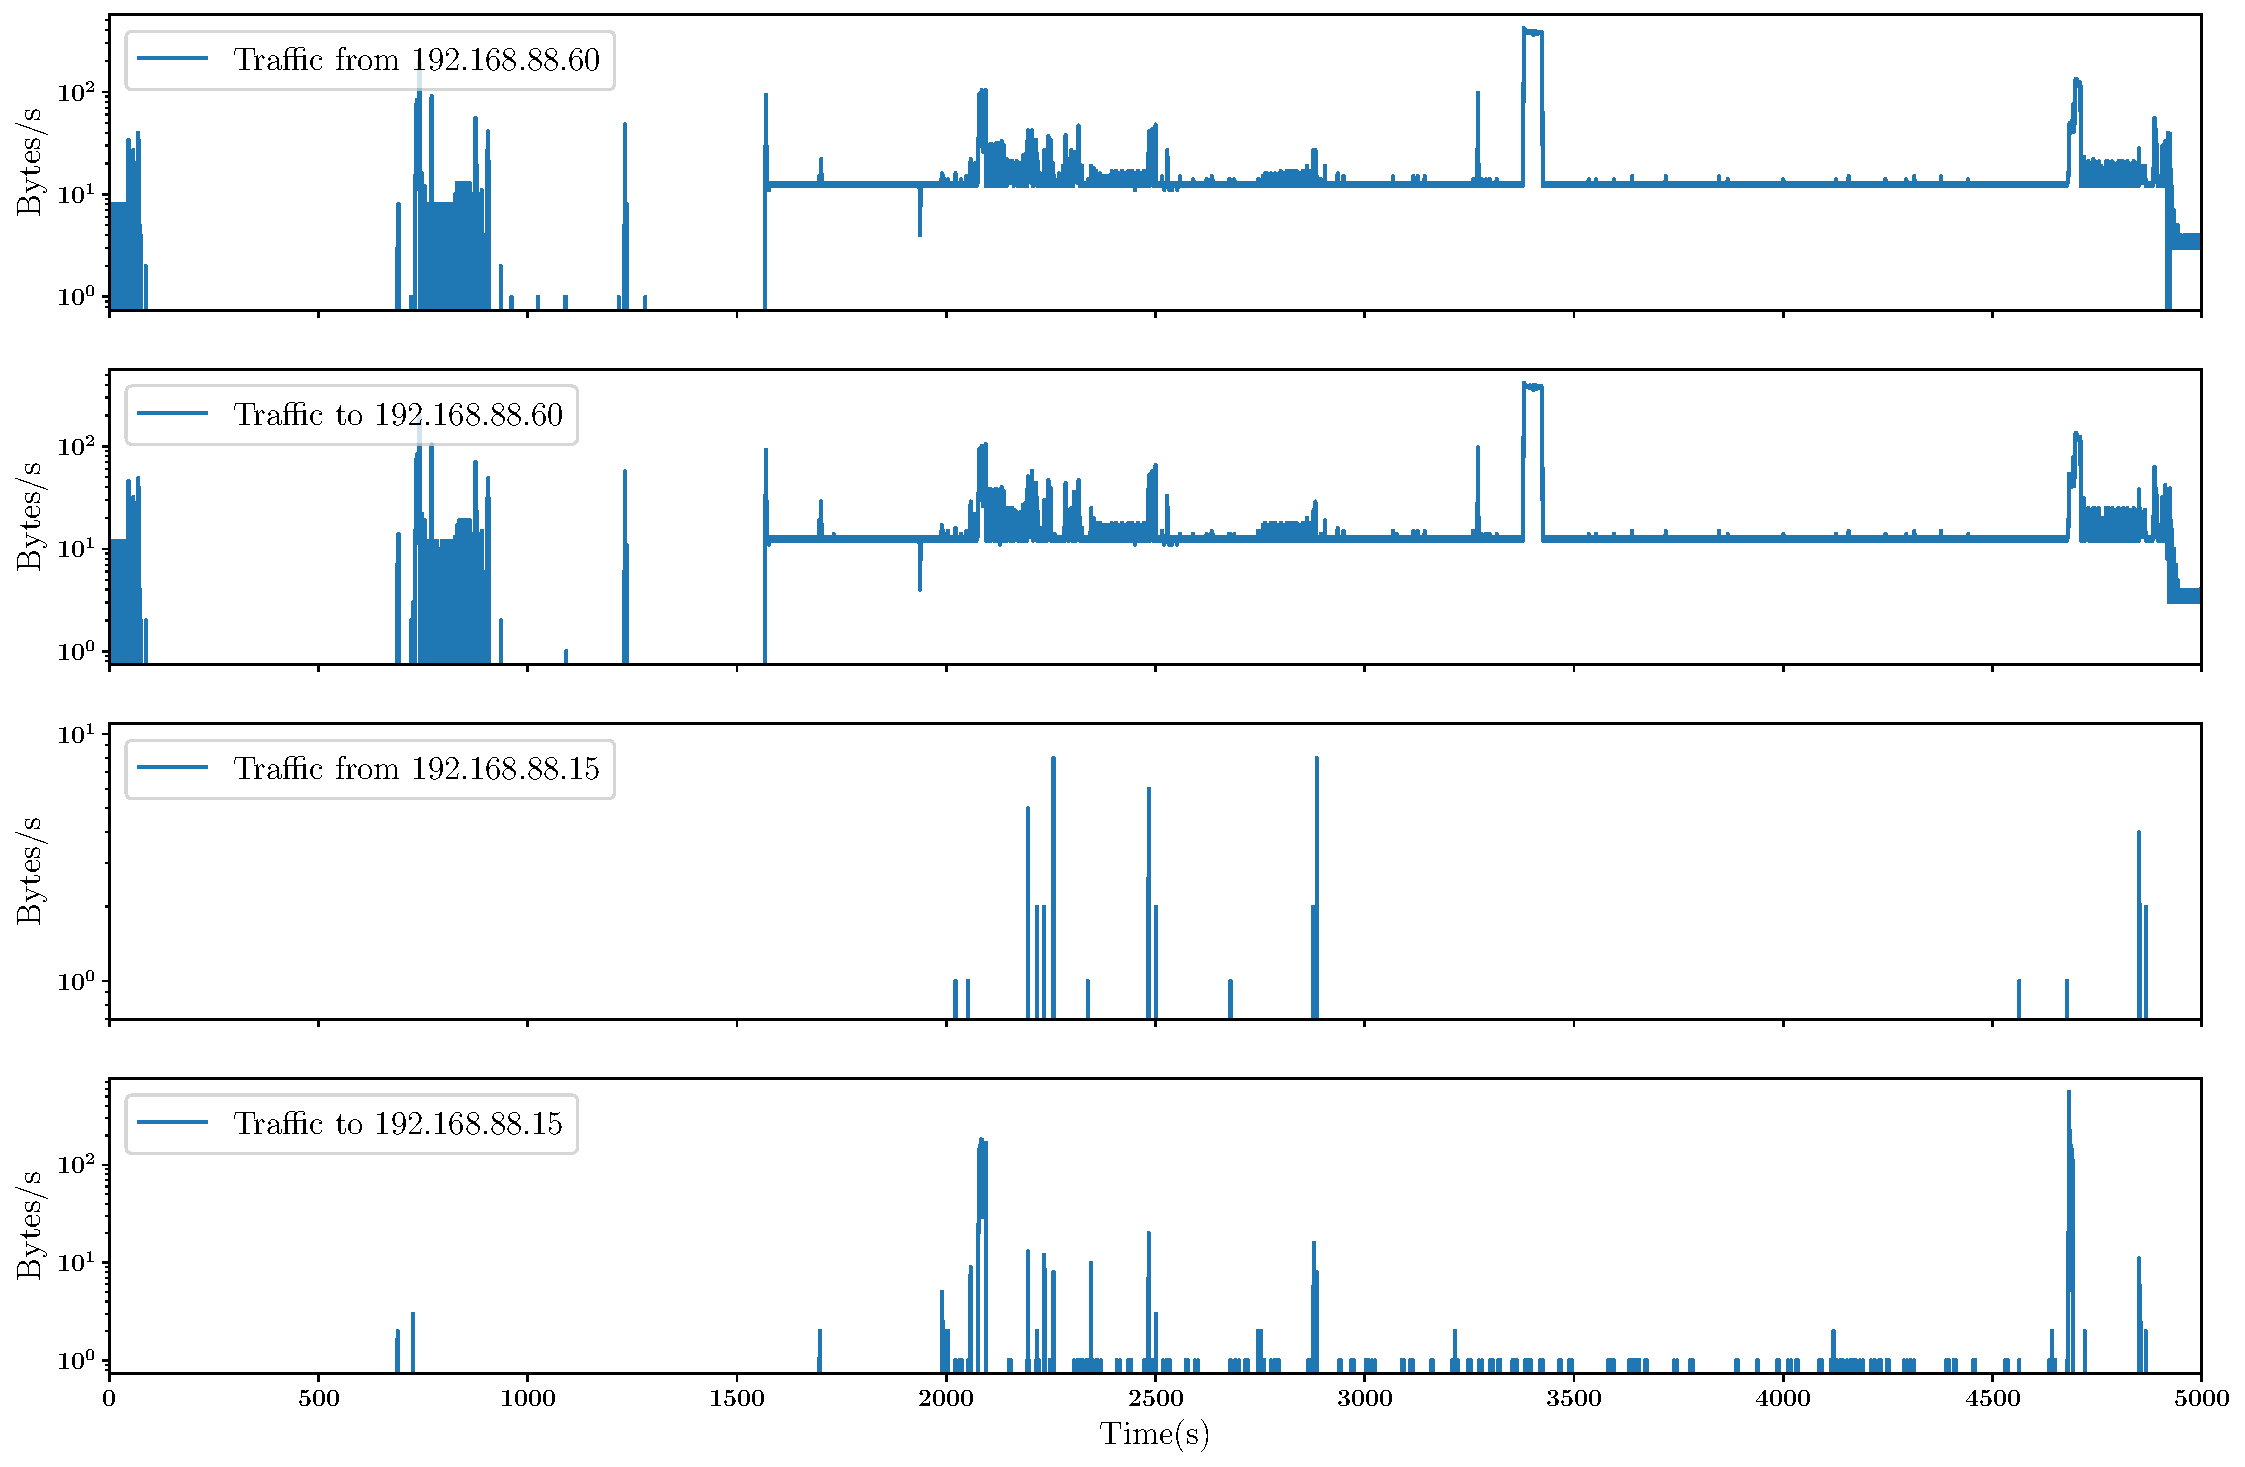
\includegraphics[width=\textwidth]{images/preprocessing/ts_4sics.pdf}
    \caption{Extracted time series from the 4SICS dataset. From top to bottom: transferred bytes from and to the Moxa EDS-508A Switch (IP address 192.168.88.60), transferred bytes from and to the DirectLogic 205 PLC (IP address 192.168.88.15).}
    \label{fig:ts_example_4sics}
    \vspace{-3mm}
\end{figure}
\begin{figure}[!h]
    \centering
       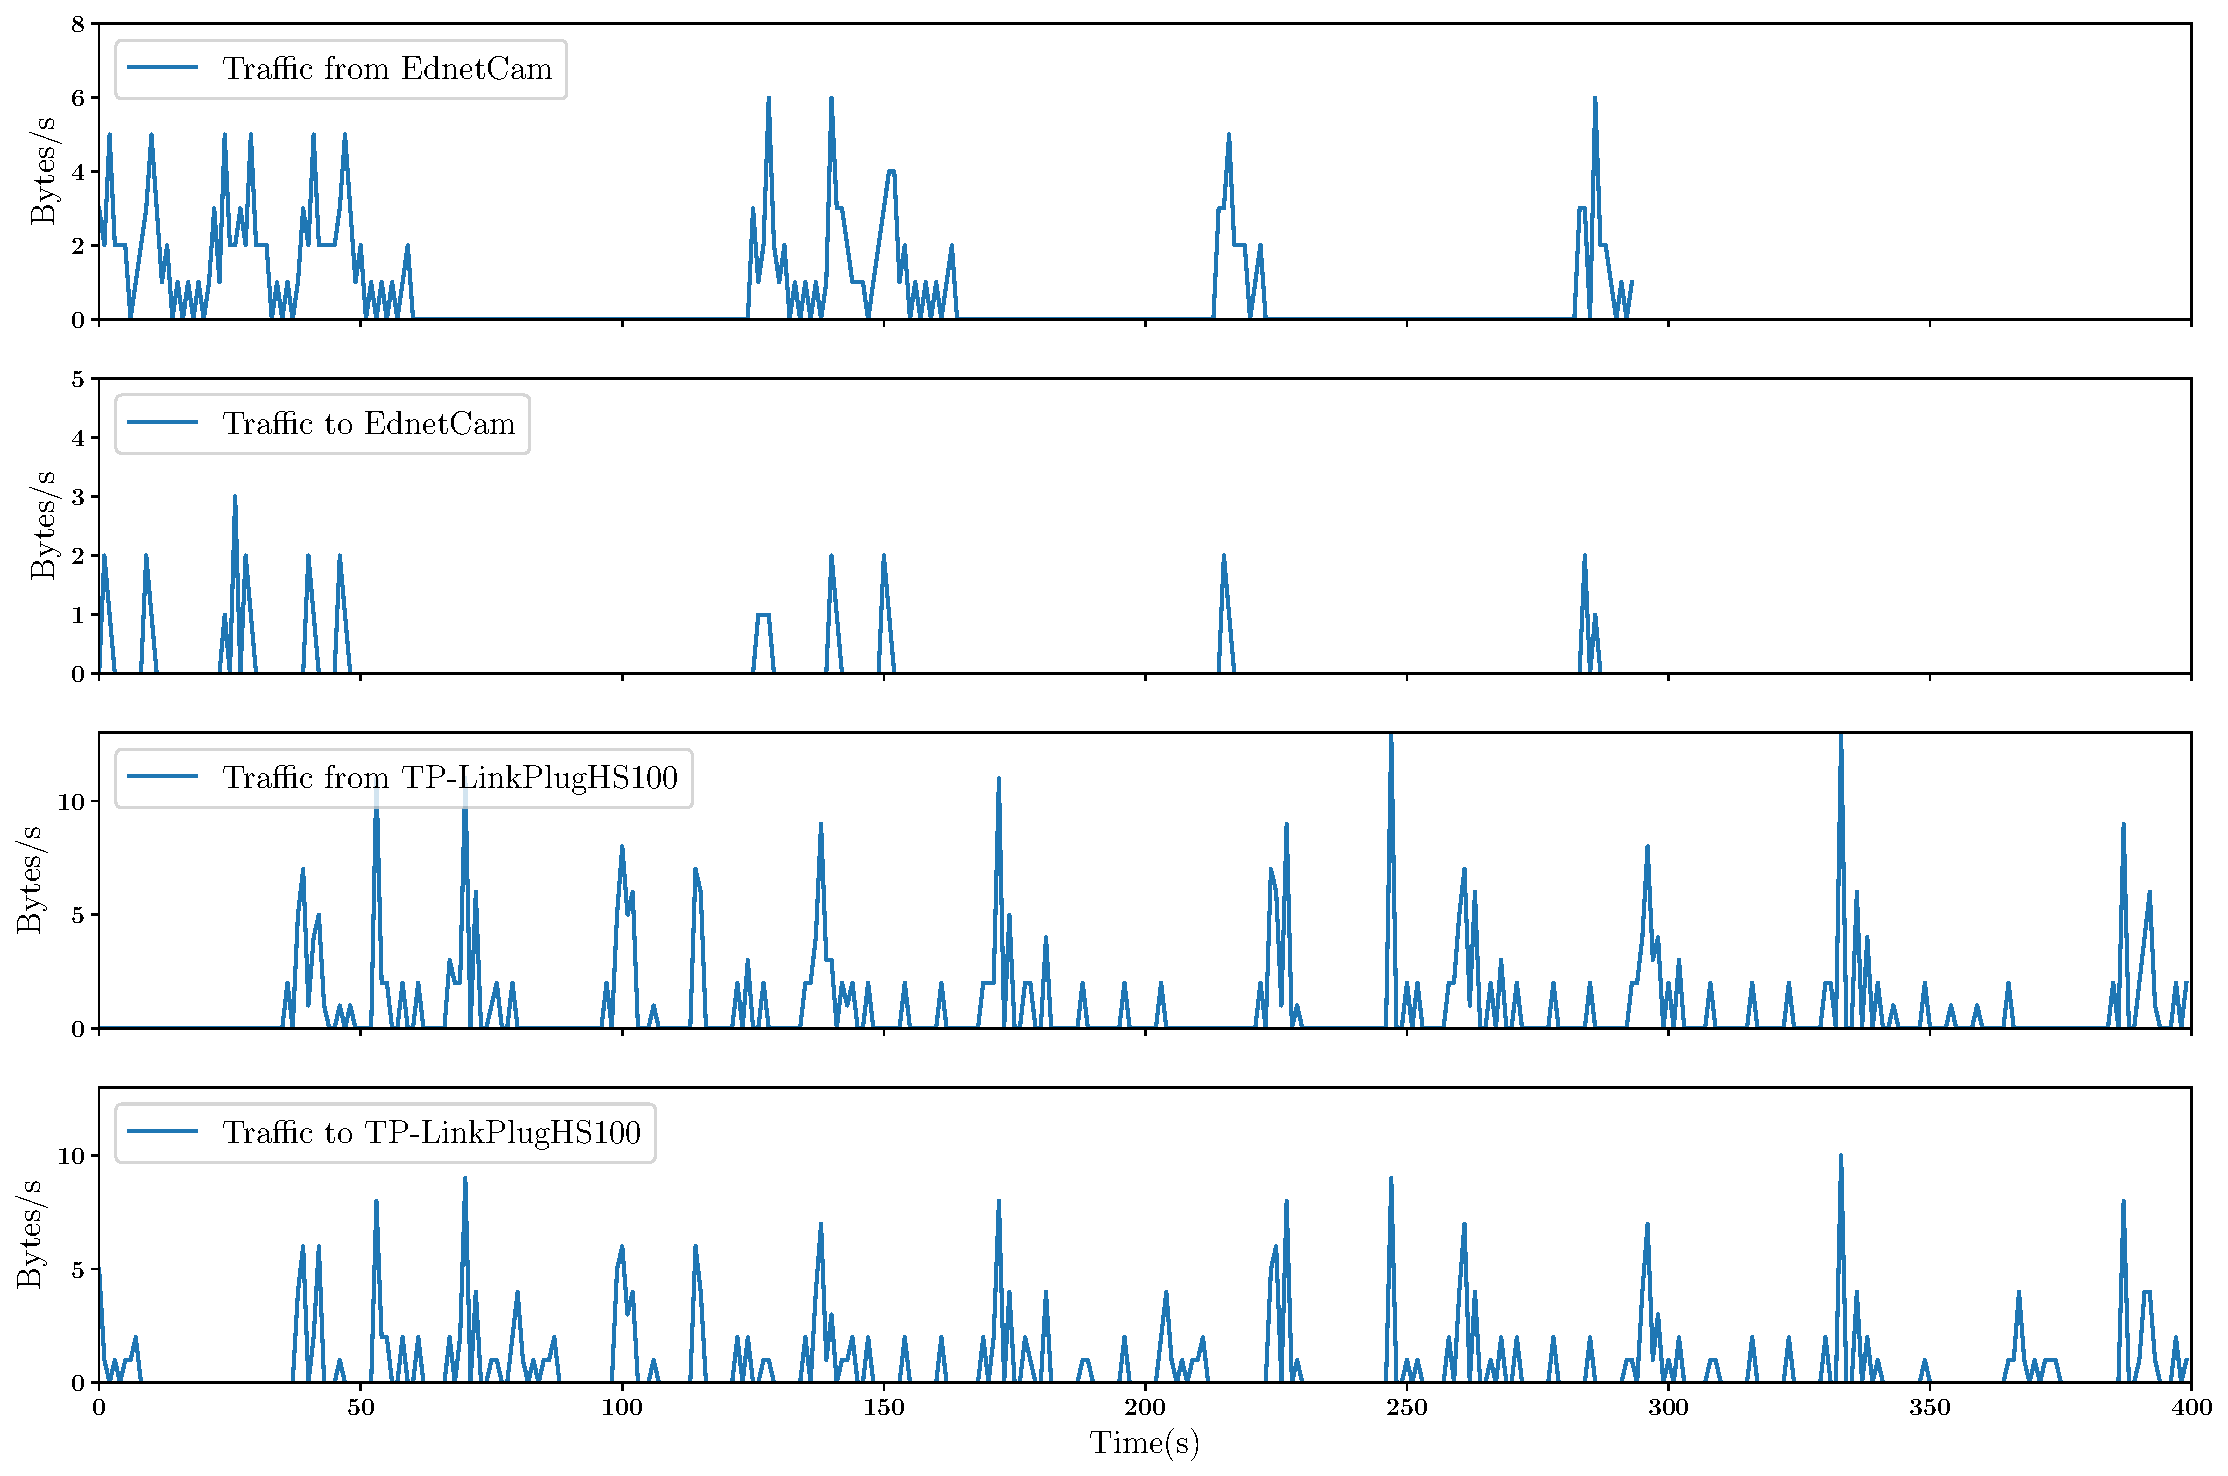
\includegraphics[width=\textwidth]{images/preprocessing/ts_iot.pdf}
    \caption{Extracted time series from the IoT sentinel dataset. From top to bottom: transferred bytes from/to the EdnetCam and from/to the TP-LinkPlugHS100.}
    \label{fig:ts_example_iot}
    \vspace{-5mm}
\end{figure}



\section{Time series preprocessing}

Despite being now saved in a simple format the extracted time series are still not utilizable as input of a classifier. There are many reasons for this, the main ones being the irregularity of the time series length and not being normalized. To solve this issue we have to preprocess the time series before utilizing them for the classification. 
The prepocessing procedure, visually represented in \figref{fig:ts_processing}, is composed of the following steps:
\begin{itemize}[noitemsep]
    \item {Length standardization} and data augmentation
    \item Time series selection and feature combination
    \item Feature normalization
\end{itemize}

\subsection{Length standardization and data augmentation}

One the most important requirement, for the use of a dataset as input of Neural Netowrk classifier, is for its elements to be of uniform dimension. As we said previously the length of an extracted time series is not regular since it depends on the amount of traffic captured for that specific device.

Given a time series ${\tilde{X}_i^j}$ of length $N$ we then split it in a group of time series of length $L$, where the variable $L$ is usually also called lookback. More specifically we can now represent each device with a group of time series $\bar{x}_i^j$ with regular length and the same number of feature as the original one:
\begin{equation}
    \bar{x}_i^j = \left\{\tilde{X}_{n\cdot i}^j, \tilde{X}_{n\cdot i +1 }^j, \dots, \tilde{X}_{n\cdot(i+1)}^j  \right\}
    \qquad\text{with }n=\frac{N}{L}
\end{equation}

A visual representation of the spliiting of time series with this method is shown in \figref{fig:ts_split_std}. This approach produces a set of $\frac{N}{L}$ time series for each device that can now be utilized as the desired input of a classifier, but is still affected by an issue. As we said before, looking at the time series shown in \figref{fig:ts_example_4sics} and \figref{fig:ts_example_iot}, we can notice that the number of elements in the IoT dataset time series is very low with most of them having less than 1000 elements. 

\begin{figure}[h]
    \centering
\includestandalone[width=0.8\textwidth]{images/preprocessing/standard_splitting}
\caption{Application of the "standard" splitting method to a mono variate time series. The original time series of length $N$ is divided in $\frac{N}{L}$ time series of length $L$.}
    \label{fig:ts_split_std}
\end{figure}

In order to achieve good performances the training set of a classifier requires a big number of training samples, usually at least the same as the number of its free parameters. As we will shown in \chapref{chap6} a value of the lookback lower $L=30$ produces time series too short for an effective training of the model. 
The combination of this approach with the necessity of using a value of $L$ at least equal to 30 results in the impossibility of creating enough samples for IoT dataset. The only way to solve this issue is to implement a data augmentation methodology during the division of the ${\tilde{X}_i^j}$ time series, namely we want to implement some technique that allows us to increase the number of time series extracted from ${\tilde{X}_i^j}$. Many possible techniques can be implemented, such as generating time series with a Monte Carlo algorithm from the $\bar{x}_i^j$ samples, but a simpler, yet very effective, technique was implemented for this work. \\
The standard splitting method divides the original time series is $\frac{N}{L}$ time series where each one has completely different temporal values than the others. It is instead possible to split the original time series in such a way that each series shares $L-1$ temporal values with the previous and subsequent one, differing by just one value. Using this approach the time series group $\bar{x}_i^j$
is now defined as:
\begin{equation}
    \bar{x}_i^j = \left\{\tilde{X}_{i}^j, \tilde{X}_{i +1 }^j, \dots, \tilde{X}_{i+L-1)}^j  \right\}
\end{equation}
A visual representation of this method for the time series splitting is shown if \figref{fig:ts_split_aug}.
This second approach leads to the creation of $N-L+1$ time series solving the issue of having too few samples for the IoT dataset. Calling with $n_S$ and $n_A$ the number of time series respectively generated with the "standard" and "data augmentation" approach, if we compute the ratio between the two, we obtain:
\begin{equation}
    \frac{n_A}{n_S} = \frac{N-L+1}{\frac{N}{L}} = \frac{N-L+1}{N}\cdot L \quad \xrightarrow{N>>L}
    \quad \frac{n_A}{n_S}= L 
\end{equation}
\begin{figure}[h]
\vspace{-7mm}
    \centering
\includestandalone[width=0.9\textwidth]{images/preprocessing/augmented_splitting}
\caption{Application of the "augmented" splitting method to a mono variate time series. The original time series of length $N$ is divided in $N-L+1$ time series of length $L$ each one sharing $L-1$ values with the previous and subsequent one.}
    \label{fig:ts_split_aug}
    \vspace{-10mm}
\end{figure}
\newpage
Considering that, as said before L must be at least bigger than 25, we can see that for big enough N we get a consistent increase of the number of time series obtained for each device. 

%\begin{figure}
%    \centering
%\includestandalone[width=0.8\textwidth]{images/preprocessing/standard_splitting}
%\caption{ts std}
%    \label{fig:ts_split_std}
%\end{figure}
%\begin{figure}[h]
%    \centering
%\includestandalone[width=0.9\textwidth]{images/preprocessing/augmented_splitting}
%\caption{Application of the "augmented" splitting method to a mono variate time series. The %original time series of length $N$ is divided in $N-L+1$ time series of length $L$ each one %sharing $L-1$ values with the previous and subsequent one.}
%    \label{fig:ts_split_aug}
%\end{figure}


\subsection{Time series selection and feature combination}

The dataset obtained using the methods described in the previous section can be utilized as the input of the classifier. Some operations however should be done in order to improve the efficiency of the training and the overall performance of the classifier.

The first possible operation over the $\bar{x}_i^j$ time series comes from a simple consideration: in most cases a device inside a network will not be in constant communication with the other devices but, most likely, will present time intervals with where no traffic from/to itself is produced. This consideration is also validated from the time series shown in \figref{fig:ts_example_4sics} and \figref{fig:ts_example_iot} where there are many visible intervals without any traffic from/to the considered devices.

A time interval where a device does not communicate will translate in a time series with all null values. Such type of time series not only does not bring any information regarding the device, but can also be an hindrance during the training procedure. The first operation is therefore the direct removal of all the null time series from the $\bar{x}_i^j$ datasets.

After the removal of the null time series we can focus directly on the features. As we said before we decided to separately extrapolate the time series of the traffic from and to a specific device in order to enhance the quantity of information passed to the classifier. The use of both the time series of the number transferred of packets and of transferred bytes is however redundant since, for most devices, they may be just directly proportional and, in case they are not, the relation between the two may difficult to understand for the classifier.
In order to enhance the quality of the information provided to the classifier we can then define a new group of time series $\bar{x}^{\prime j}_i$:
\begin{equation}
    \bar{x}^{\prime j}_i = 
    \begin{cases}
    \begin{aligned}
    & \bar{x}_i^j               &&\text{if}&& j&=&1,2 \\
    & \bar{x}_i^3 + \bar{x}_i^4 &&\text{if}&& j&=&3 \\
    & \bar{x}_i^3 - \bar{x}_i^4 &&\text{if}&& j&=&4 \\
    \end{aligned}
    \end{cases}
\end{equation}

With this transformation we leave untouched the information regarding the number of transferred packages, but we substitute the transferred bytes from and to a device with the total transferred bytes and the difference between transferred and received ones, removing the redundancy in the information.

\subsection{Feature normalization}

The last step of the time series preprocessing is the feature normalization. In this step we rescale the time series in order for them to have null mean and unitary variance. This step is particularly important in order to standardize the time series themselves. The main reason for the importance of this step derives from its ability of removing an eventual bias that may be introduced by external factors such as the bandwidth or the connection speed of the particular network we are considering. \\
From a mathematical point of view, the normalization translates in the definition of a new group of time series $\bar{z}^{j}_i$, computed starting from the previously defined $\bar{x}^{\prime j}_i$. Indicating with $\bar{x}^{\prime j}_{i,k}$ the k-th value of the $\bar{x}^{\prime j}_i$ time series it is possible to compute the mean value $\mu_i^j$ and standard deviation $\sigma_i^j$ of each time series as:
\begin{equation}
\mu_i^j = \frac{1}{L}\sum_{k=0}^{L-1} \bar{x}^{\prime j}_i\qquad
    \sigma_i^j = \sqrt{\frac{1}{L}\sum_{k=0}^{L-1}
                \left(\bar{x}^{\prime j}_i-\mu_i^j\right)}
\end{equation}
The normalized time series $\bar{z}^{j}_i$ is then defined as :
\begin{equation}
    \bar{z}^{j}_i = \frac{\bar{x}^{\prime j}_i - \mu_i^j}{\sigma_i^j}
\end{equation}
After the application of the normalization procedure over the selected and modified time series we now have a standardized representation of each device which can be used to train a Neural Network classifier. A visual summary of all the steps of the preprocessing procedure in shown in \figref{fig:ts_processing}.



\begin{figure}
    \centering
\includestandalone[width=\textwidth]{images/networks/ts_processing_v1}
%\includestandalone[width=\textwidth]{images/networks/ts_processing_v2}
\caption{Graphical representation of the preprocessing procedure over a mono variate time series. The steps, represented from left to right are: time series splitting, removal of the null time series and normalization of the cleaned dataset.}
    \label{fig:ts_processing}
\end{figure}

\section{Communication protocol analysis}

The analysis of traffic time series is by itself enough to train a classifier able to perform the identification task up to a certain level of accuracy. The use of only the time series itself is however reductive in the representation of a device and does not exploit all the information that we can extrapolate from a traffic file.

As previously described we are interested in performing an identification of the devices without using the "standard" identifiers provided by the devices themselves. However an important information, that we are not yet exploiting during the analysis of the time series, is the protocol used by a device to communicate with the others.
The use of the information regarding the communication protocols used by a device may improve significantly the capability of a classifier to identify a device and should therefore be included in the representation of the device.
The first step is then to associate each device with a list of all the protocol used to communicate, this operation is done using the Guardian Community Edition(GCE) and analysing the \texttt{pcap} files with it. The simple association of a device with all the protocols used to communicate is however not directly usable as information for a classifier since it requires the information to be in a numeric format.

The simplest way to convert this list to a numeric input would then be: enumerate the list of all protocols used in a traffic file and associate each device with a vector containing the indices of the used protocols. However, similarly to the use of a full length time series, this approach is not optimal due to the non regular length of the generated vector, since the number of used protocols changes with each device. Considering also the big variety of protocols and the fact that in the future many other protocols will be developed and implemented the use of this approach will not lead to a good representation of the device.
A better approach is to divide the communication protocols in classes based on the high level behaviour of a communication done via that protocol, namely we want to group protocols used for the same type of operations together. Once the classes are defined we can associate each device to a vector of binary values with the same length of the number of classes, where each binary value is either 1, if the device uses a protocol of a specific class, or 0, if the other case. This approach offers many advantages, the first one being an already optimal input for the training of a classifier, since the vectors have regular length and standardized values. More importantly, this approach allows the generalization to new protocols by just adding them to the specific class.

To better illustrate this approach let's make an example. Let's for simplicity define only three classes of protocols:
\begin{itemize}[noitemsep, nolistsep]
    \item \textbf{OT protocols}: \texttt{dnp3}, \texttt{modbus}
    \item \textbf{Monitoring}: \texttt{snmp}, \texttt{igmp}, \texttt{s7}
    \item \textbf{Applications}: \texttt{imap}, \texttt{pop3}, \texttt{https}
\end{itemize}
If we then have a device associated to the following list of protocols: \texttt{"dnp imap pop3 https"}, we will represent it with $[1,0,1]$ since it uses OT and application protocols but not monitoring ones.
In \tabref{tab:protolist} a list of the classes of communication protocols considered in this work is reported.


\section{Dataset division and device classes}

In the previous sections we described how to extrapolate useful information from a traffic file and how to process it in order to represent a specific device. Looking at the dataset device table, \tabref{tab:4sicsdataset} and \tabref{tab:iotdataset}, we can see that there are many similar devices, such as switches or sensors. 
To further enhance the capability of identifying a device we can therefore group similar devices in classes allowing the classifier to be trained on a more varied and bigger dataset, resulting in a more robust classifier. This choice has also the great advantage of enhancing the capability of identifying devices that are not part of the training dataset, which translate it the eventual capability of identifying also devices that will be developed in the future without needing to retrain the classifier.
\begin{table}[h]
\centering
\begin{tabular}{|l|l|}
\hline
\textbf{Class} & \textbf{Communication protocols} \\
\hline
OT protocols   &  dnp3 ,  modbus ,  ethernetip ,   pi-connect \\
Authentication & kerberos ,  netbios-ns ,  dce-rpc ,  kms \\
Base           & dns ,  mdns ,  ssdp \\
Monitoring     & snmp ,  igmp ,  s7 ,  ldaps ,  vnc ,  ssh \\
Data Transfer  & ftp ,  tcp ,  ip ,  netbios-ssn ,  udp ,  ftps ,  cotp ,   ftps-data \\
Applications   & browser ,  http ,  https ,  telnet ,    dropbox-lsp ,  smtp ,  imap ,  imaps ,  pop3  \\
\hline
\end{tabular}
\caption{List of communications protocols considered for the analysis. Protocols are grouped in class depending on their high level behaviour.}
\label{tab:protolist}
\end{table}


We now have all the ingredients needed to create our training dataset. One last thing that is important to mention is that the training dataset, as in most the Machine Learning applications,
does not correspond to the full dataset. The full dataset, composed of the $\bar{z}_j^j$ time series and the protocol communication binary vectors, is in fact split in three subsets:
\begin{itemize}[noitemsep, nolistsep]
    \item \textbf{Training set}: the set used in the training procedure to train the classifier, the best parameters of the model are estimated to minimize the loss over this set
    \item \textbf{Validation set}: used during the training to monitor the model accuracy and of  loss function in order to identify the eventual presence of an overfitting behaviour 
    \item \textbf{Test set}: used after the training to evaluate the real model accuracy of the model
\end{itemize}
For each device the subsets are randomly created using the 60\% of the total number of samples for the training set and the 20\% for both the validation and test set.
The devices used to create the final datasets, grouped by device classes, alongside with the number of sample assigned to each subset, are reported in \tabref{tab:4sicsdev} and \tabref{tab:iotdev}.




\begin{table}[h]
\centering
\begin{tabular}{llrrrr}
\toprule
\textbf{Device Class} & \textbf{Devices} & \multicolumn{4}{c}{\textbf{Number of samples}} \\
& & Training & Validation & Test & Total \\
\midrule
\multirow{1}{*}{PLC} & Siemens SIMATIC S7-1200 & 6426 & 2143 & 2143 & 10712  \\
                     & xLogic x-Messenger & 3572 & 1192 & 1192 & 5956  \\
\midrule
\multirow{1}{*}{Camera}  & AXIS 206 & 6679 & 2227 & 2227 & 11133 \\
\midrule
\multirow{1}{*}{Switch$^*$} & Moxa EDS-508A  & 9000 & 3000 & 3000 & 15000 \\
\midrule
\multirow{1}{*}{Firewall}& Hirchmann EAGLE 20 Tofino & 3903 & 1301 & 1301 & 6505 \\
\midrule
\multirow{1}{*}{Router$^*$} & Westermo Lynx 3643-0105  & 9000 & 3000 & 3000 & 15000  \\ 
\midrule
\midrule
Total & & 38584 & 12861 & 12861 & 64306 \\
\bottomrule
\end{tabular}
\caption{Device used for the creation of the final 4SICS dataset for the device identification, grouped by device type.}
\label{tab:4sicsdev}
\end{table}



\begin{table}[t]
\centering
\begin{tabular}{llrrrr}
\toprule
\textbf{Device Class} & \textbf{Devices} & \multicolumn{4}{c}{\textbf{Number of samples}} \\
& & Training & Validation & Test & Total \\
\midrule
\multirow{3}{*}{Camera}  & D-LinkCam     & 1348 & 449 & 449 & 2246  \\
                         & D-LinkDayCam  & 332 & 110 & 110 & 552  \\
                         & EdnetCam      & 105 & 35 & 35 & 175  \\
\midrule
\multirow{2}{*}{Light Switch} & HueSwitch & 1396 & 466 & 466 & 2328 \\
                             &  WeMoInsightSwitch & 830 & 342 & 342 & 1714  \\
\midrule
\multirow{3}{*}{Sensor} &  D-LinkSensor  & 1056 & 352 & 352 & 1760 \\
                         & D-LinkDoorSensor  & 1100 & 366 & 366 & 1832  \\
                         & D-LinkWaterSensor  & 1184 & 394 & 394 & 1972  \\
\midrule
\multirow{4}{*}{Smart Plug}& D-LinkSwitch  & 1113 & 371 & 371 & 1855 \\
                          & EdimaxPlug1101W & 806 & 269 & 269 & 1344  \\
                          & HomeMaticPlug & 449 & 150 & 150 & 749  \\
                          & TP-LinkPlugHS110 & 457 & 140 & 140 & 697  \\
\midrule
\midrule
Total & & 12056 & 2584 & 2584 & 17224 \\
\bottomrule
\end{tabular}
\caption{Device used for the creation of the final IoT Sentinel dataset for the device identification, grouped by device type. Statistics regarding the number of samples in each subset, after the preprocessing procedure, is also reported.}\label{tab:iotdev}
\vspace{12cm}
\end{table}


